\subsection{Client/server model}%
\label{sec:client-serv-model}
The client/server model is the most common form of network architecture used
in data communications today~\cite{hanson2000client}. A client is a system or
application that request the activity of a service provider system or
application, called servers, to accomplish specific tasks.
The client/server concept functionally divides the execution of a unit
of work between activities initiated by the end user (client) and resource responses
(services) to the activity request as a cooperative environment~\cite{hanson2000client}. The client,
typically handling user interactions and data exchange/modification in the user’s
behalf, makes a request for a service, and a server, often requiring some resource
management (synchronization and access to the resource), performs that service,
responding to the client requests with either data or status information~\cite{ibmCliServ}.

An example of a simple client-server model using the Socket \gls{api}, through system
calls, is presented in Fig.~\ref{fig:cli-serv-operation}. The operation of sockets can be explained as
follows~\cite{kerrisk2010linux}:
\begin{itemize}
\item The \texttt{socket()} system call creates a new socket, establishing the
  protocols under which they should communicate. For both client and server to
communicate, each of them must create a socket.
\item  Communication via a stream socket is analogous to a telephone call. One
application must connect its socket to another application’s socket before
communication can take place. Two sockets are connected as follows:
\begin{enumerate}
\item One application, assuming the role of server, calls \texttt{bind()} to
  bind the socket to a well-known address, and then calls \texttt{listen()} to
  notify the kernel it is ready to accept incoming connections.
\item The other application, assuming the role of client, establishes the
  connection by calling \texttt{connect()}, specifying the address of the socket
  to which the connection is to be made.
\item The server then accepts the connection using \texttt{accept()}. If the
  \texttt{accept()} is performed before the client application calls
  \texttt{connect()}, then the \texttt{accept()} blocks.
\end{enumerate}
\item Once a connection has been established, data can be transmitted in both
directions between the applications (analogous to a bidirectional telephone
conversation) until one of them closes the connection using \texttt{close()}.
\item Communication is performed using the conventional \texttt{read()} and
  \texttt{write()} system calls or via a number of socket-specific system calls
  (such as \texttt{send()} and \texttt{recv()}) that provide additional
  functionality. By default, these system calls block if the \gls{io} operation
  can’t be completed immediately. However, nonblocking \gls{io} is also
  possible.
\end{itemize}
% Overview of UNIX system calls
\begin{figure}[!hbt]
\centering
    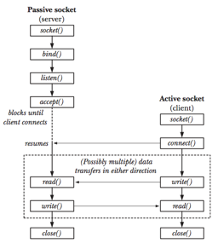
\includegraphics[width=0.4\textwidth]{./img/cli-serv-operation.png}
  \caption{Overview of UNIX system calls with sockets implementing 
a server/client paradigm (withdrawn from~\cite{kerrisk2010linux})}%
\label{fig:cli-serv-operation}
\end{figure}
%
%%% Local Variables:
%%% mode: latex
%%% TeX-master: "../../../dissertation"
%%% End:
